% What X-Forge works with. Build: tectonic support.tex (or pdflatex), then
%   dvisvgm --pdf support.pdf -o support.svg
\documentclass[tikz,border=8pt]{standalone}
\usepackage[T1]{fontenc}
\usepackage{lmodern}

\definecolor{ok}{HTML}{E4F2DF}   \definecolor{okline}{HTML}{4A7F3A}
\definecolor{part}{HTML}{FFF4DC} \definecolor{partline}{HTML}{B7862B}
\definecolor{band}{HTML}{F7F7F7}

\tikzset{
  chip/.style={rounded corners=3pt, minimum height=10mm, text width=#1, align=center,
               font=\sffamily\small, line width=0.8pt},
  chip/.default=26mm,
  ok/.style={chip=#1, fill=ok, draw=okline},     ok/.default=26mm,
  part/.style={chip=#1, fill=part, draw=partline}, part/.default=26mm,
  plan/.style={chip=#1, fill=white, draw=black!50, dashed}, plan/.default=26mm,
  label/.style={font=\sffamily\bfseries, anchor=west, align=left},
  sub/.style={font=\sffamily\scriptsize, text=black!65},
}

% \row{y}{title}{subtitle}: a band with its label at height y (cm)
\newcommand{\row}[3]{%
  \fill[band, rounded corners=4pt] (-0.3,#1-0.75) rectangle (21.4,#1+0.75);
  \node[label] at (0,#1) {#2\\[-1pt]{\mdseries\scriptsize\color{black!65}#3}};}

\begin{document}
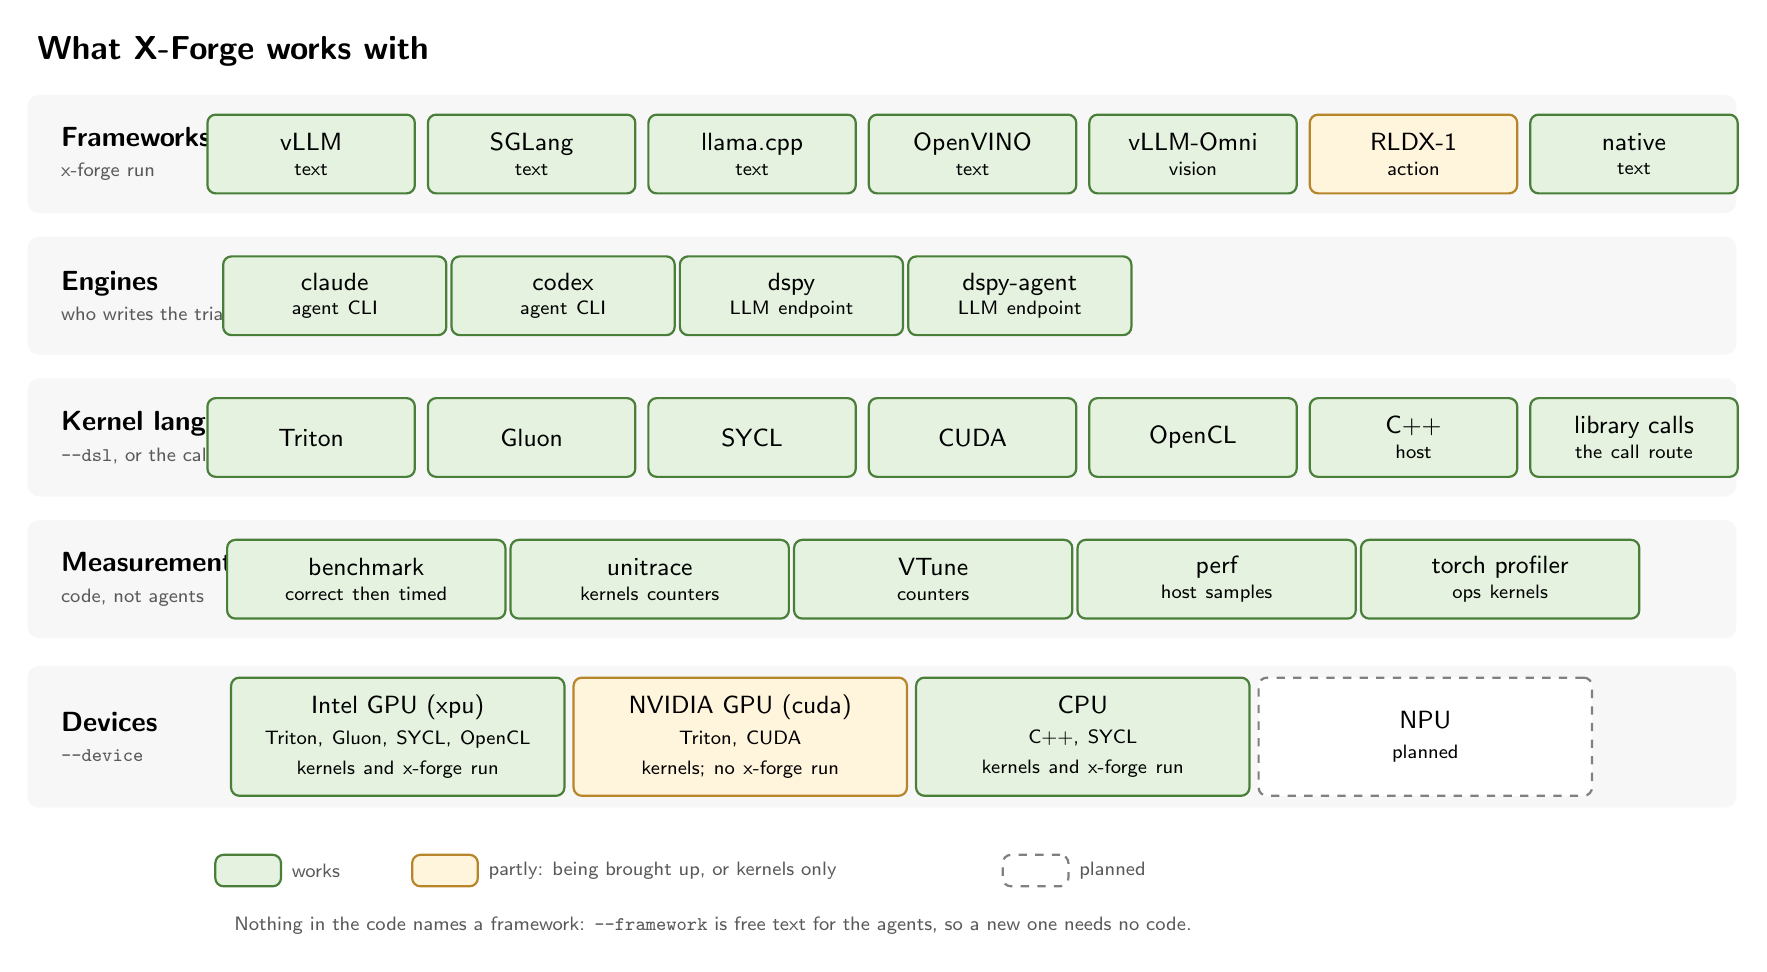
\begin{tikzpicture}[x=1cm, y=1cm]
\node[font=\sffamily\bfseries\large, anchor=west] at (-0.3,1.3) {What X-Forge works with};

\row{0}{Frameworks}{x-forge run}
\foreach \n/\w [count=\i] in {vLLM/text, SGLang/text, llama.cpp/text, OpenVINO/text, vLLM-Omni/vision}
  \node[ok=24mm] at (3.3+2.8*\i-2.8, 0) {\n\\[-2pt]{\scriptsize \w}};
\node[part=24mm] at (3.3+2.8*5, 0) {RLDX-1\\[-2pt]{\scriptsize action}};
\node[ok=24mm] at (3.3+2.8*6, 0) {native\\[-2pt]{\scriptsize text}};

\row{-1.8}{Engines}{who writes the trials}
\foreach \n/\w [count=\i] in {claude/agent CLI, codex/agent CLI, dspy/LLM endpoint, dspy-agent/LLM endpoint}
  \node[ok] at (3.6+2.9*\i-2.9, -1.8) {\n\\[-2pt]{\scriptsize \w}};

\row{-3.6}{Kernel languages}{\texttt{--dsl}, or the call route}
\foreach \n [count=\i] in {Triton, Gluon, SYCL, CUDA, OpenCL}
  \node[ok=24mm] at (3.3+2.8*\i-2.8, -3.6) {\n};
\node[ok=24mm] at (3.3+2.8*5, -3.6) {C++\\[-2pt]{\scriptsize host}};
\node[ok=24mm] at (3.3+2.8*6, -3.6) {library calls\\[-2pt]{\scriptsize the call route}};

\row{-5.4}{Measurement}{code, not agents}
\foreach \n/\w [count=\i] in {benchmark/correct then timed, unitrace/kernels counters,
                              VTune/counters, perf/host samples, torch profiler/ops kernels}
  \node[ok=33mm] at (4.0+3.6*\i-3.6, -5.4) {\n\\[-2pt]{\scriptsize \w}};

\fill[band, rounded corners=4pt] (-0.3,-8.3) rectangle (21.4,-6.5);
\node[label] at (0,-7.4) {Devices\\[-1pt]{\mdseries\scriptsize\color{black!65}\texttt{--device}}};
\node[ok=40mm, minimum height=15mm]   at (4.4, -7.4)
  {Intel GPU (xpu)\\{\scriptsize Triton, Gluon, SYCL, OpenCL}\\{\scriptsize kernels and x-forge run}};
\node[part=40mm, minimum height=15mm] at (8.75, -7.4)
  {NVIDIA GPU (cuda)\\{\scriptsize Triton, CUDA}\\{\scriptsize kernels; no x-forge run}};
\node[ok=40mm, minimum height=15mm]   at (13.1, -7.4)
  {CPU\\{\scriptsize C++, SYCL}\\{\scriptsize kernels and x-forge run}};
\node[plan=40mm, minimum height=15mm] at (17.45, -7.4) {NPU\\{\scriptsize planned}};

\node[ok=6mm, minimum height=4mm] (a) at (2.5,-9.1) {};
\node[sub, anchor=west] at (a.east) {works};
\node[part=6mm, minimum height=4mm] (b) at (5,-9.1) {};
\node[sub, anchor=west] at (b.east) {partly: being brought up, or kernels only};
\node[plan=6mm, minimum height=4mm] (c) at (12.5,-9.1) {};
\node[sub, anchor=west] at (c.east) {planned};
\node[sub, anchor=west] at (2.2,-9.8) {Nothing in the code names a framework: \texttt{--framework} is
  free text for the agents, so a new one needs no code.};
\end{tikzpicture}
\end{document}
